\chapter{Patterns Discussion}

	\section{Why Patterns}
		A pattern describes both a problem which occurs over and over again and
		the core of the solution to that problem. This solution can be used
		whenever this or a similar problem exists. Patterns can be combined and are 
		therefore a valuable design strategy for large applications. There are many advantages
		of using patterns over a classical design. The scope of this thesis is not to 
		list all of the advantages but to talk about specific patterns which are worth studying
		for this purpose.
		
		Not all of the following patterns describe a technically complex problem but they
		give a vocabulary to talk about problems in a manner which everybody understands
		easily who knows this vocabulary.
		
	\section{Which Patterns}
		There exists thousands of patterns out there. Not all patterns are relevant
		for a given application, in fact, a minority is. This raises the problem
		of choosing the patterns, which should be done carefully because it directly
		affects the application's design.

		The following list is a summary of all patterns relevant for this thesis. They are 
		mainly taken from M. Fowler \cite{Fowler03}. The list is in alphabetical order.
		\LTXtable{\linewidth}{./files/inc/tables/patternsUsedPatterns}

	\section{Describe the Patterns}
		Of course, one needs to know what a pattern at the end does and which
		benefits it provides. First, each pattern mentioned in the last section will 
		be described separately before they are put in a big context. The following 
		description is not meant as a complete reference but as a short description
		of each relevant pattern. Especially implementation details are left aside. They will be
		addressed in further chapters. Event though, this description should give enough information to understand
		what each pattern is for. For a more detailed discussion of these patterns, please read
		M. Fowler's Patterns of Enterprise Application Architecture \cite{Fowler03}.
		
		\subsection{Domain Model}
		\label{subsec:domainModel}
			The domain model pattern essentially describes that the domain layer
			is organised in an object-oriented (OO) manner. This technique is commonly
			used and understood and therefore not described in further detail. 
			
		\subsection{Service Layer}
		\label{subsec:serviceLayer}
			Enterprise applications often have different interfaces which provide access to
			business logic and data they store. Common interfaces are those for web-services,
			user interfaces, data loader, etc. A \textit{Service Layer} defines a boundary to
			the application and available operations (see Figure \ref{fig:patternsServiceLayer}). 
			Therefore, it encapsulates the application's business logic. To separate business 
			logic from the client interfaces has several advantages. First, the interface and therefore all
			possible operations are well defined and relatively easy to use for clients. Second,
			it reduces the burden of multiple implementations of the same functionality and improves code
			maintainability. A \textit{Remote Facade} (\ref{subsec:remoteFacade}) is an 
			example of a \textit{Service Layer}.
			
			\begin{figure}[htb]
				\begin{center}
					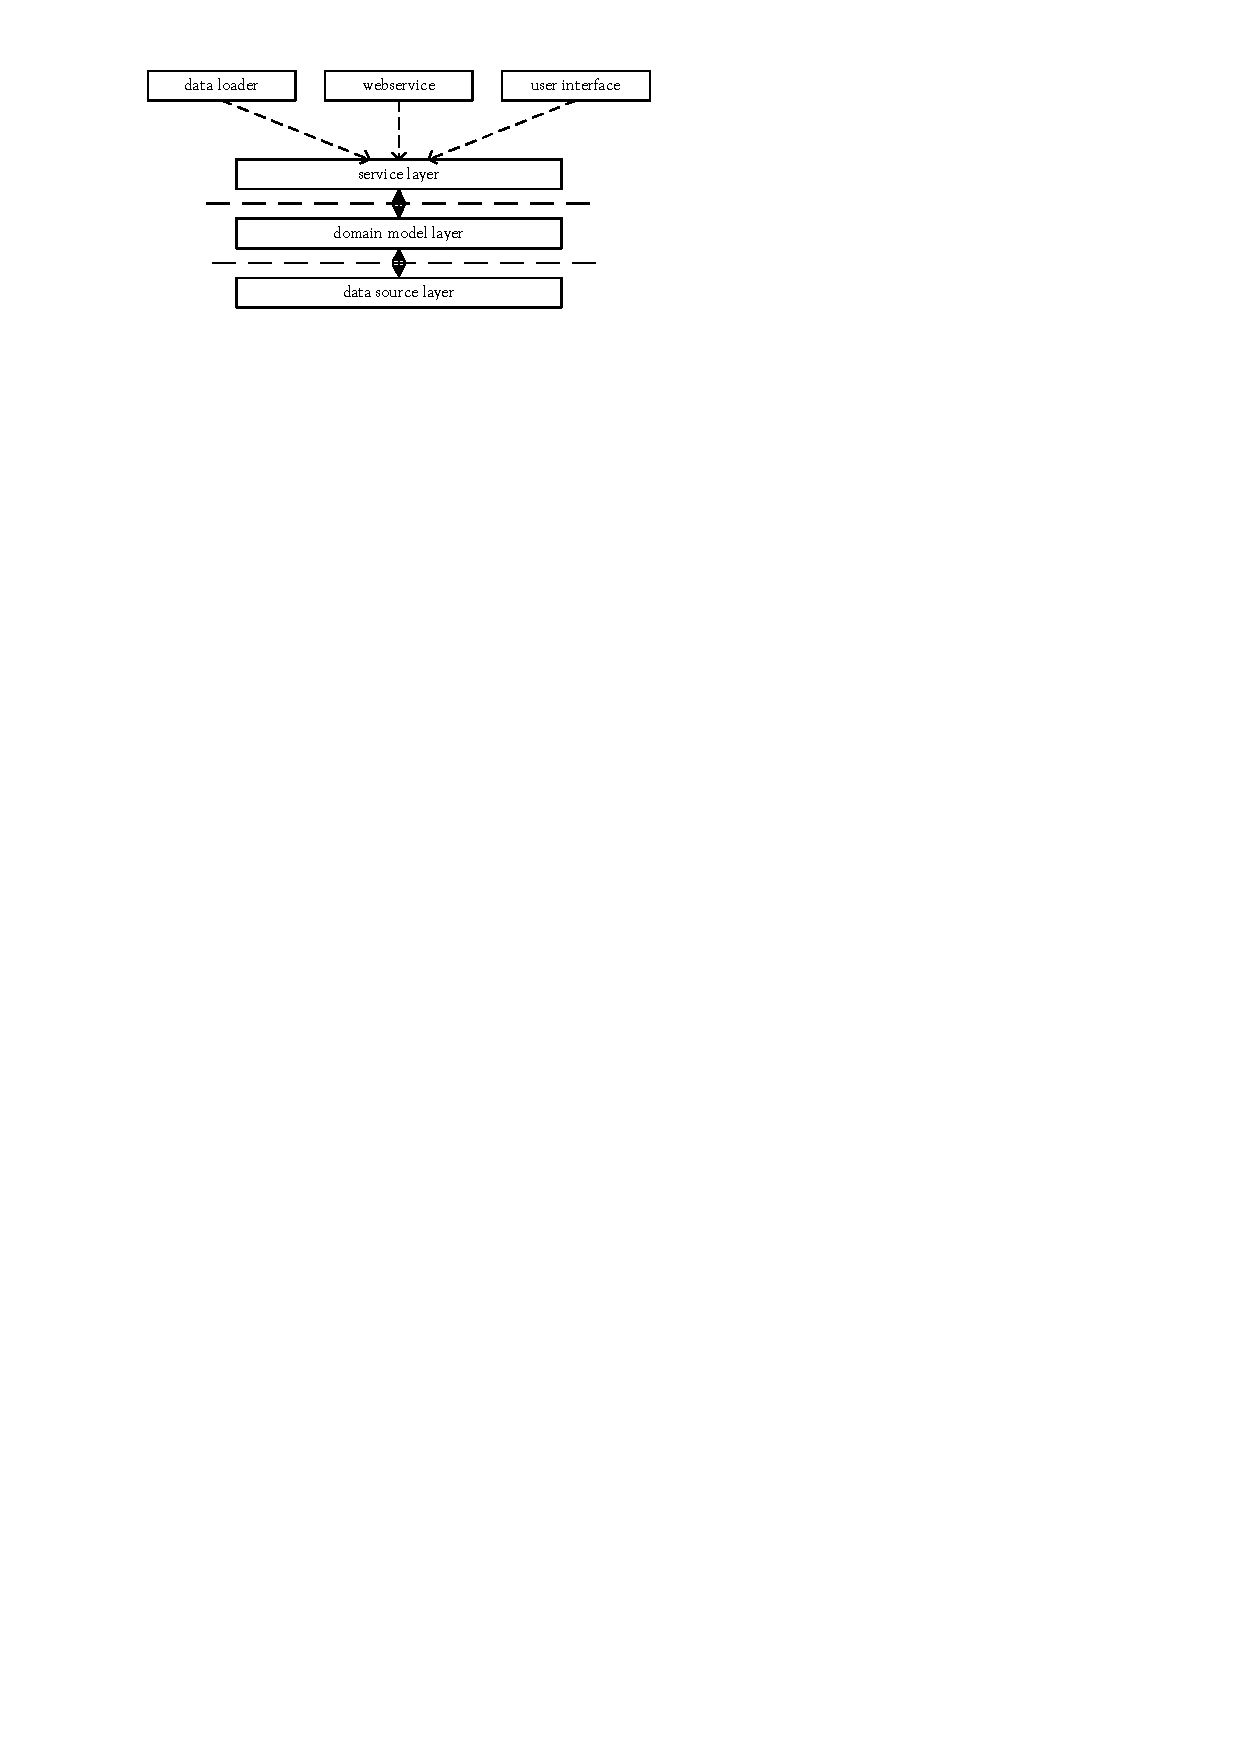
\includegraphics{./files/inc/figures/patternsServiceLayer}
					\caption{\label{fig:patternsServiceLayer} Service Layer defines application's boundary}
				\end{center}
			\end{figure}
	
		\subsection{Data Mapper}
		\label{subsec:dataMapper}
			A \textit{Data Mapper} is a layer between Domain Objects and a Database.
			A \textit{Data Mapper} is used because Objects and a relational database have
			different mechanisms for structuring data. The \textit{Data Mapper} separates in-memory objects 
			from the database and transfers data between the two. With this pattern,
			the in-memory objects do not need to know about the database at all. Figure
			\ref{fig:patternsDataMapperOverview} shows the general idea of a \textit{Data Mapper}.

			\begin{figure}[htb]
				\begin{center}
					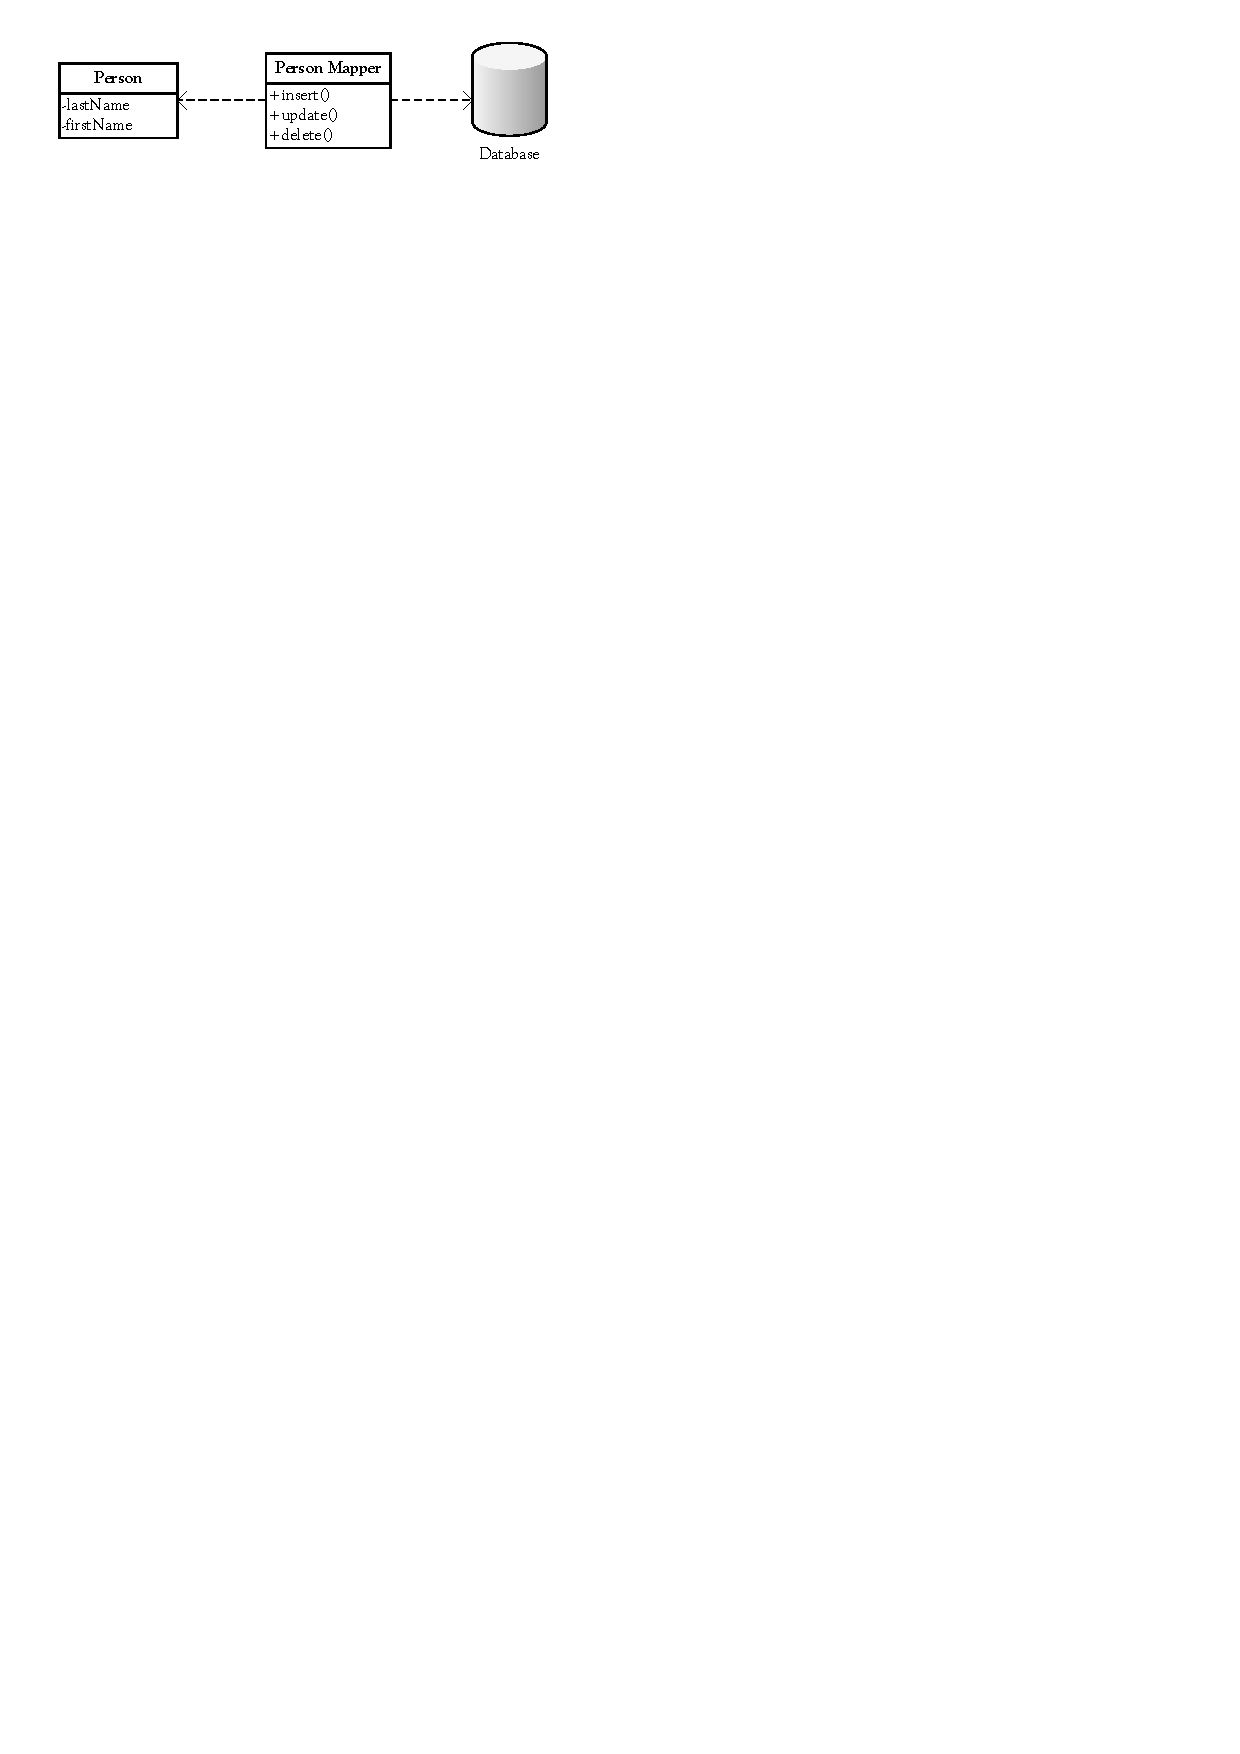
\includegraphics{./files/inc/figures/patternsDataMapperOverview}
					\caption{\label{fig:patternsDataMapperOverview} Data Mapper Overview}
				\end{center}
			\end{figure}
			The whole layer of \textit{Data Mapper} can be substituted, either for testing purposes
			or to allow a single domain layer to work with different kind of databases. This
			becomes very powerful if a \textit{Data Mapper} is combined with other patterns. This topic
			will be addressed in later chapters.
			
		\subsection{Identity Map}
		\label{subsec:identityMap}
			The basic idea behind \textit{Identity Map} is to have a series of maps containing objects
			that have been pulled from the database. If you load an object from the database,
			you first check the maps. If there already is an object which corresponds to the
			one you are loading, you do not need to load it. This is illustrated in Figure
			\ref{fig:patternsIdentityMap} 

			How many maps are needed depends on the application. You can either choose one
			map per class or one map for the whole session. 

			\begin{figure}[htb]
				\begin{center}
					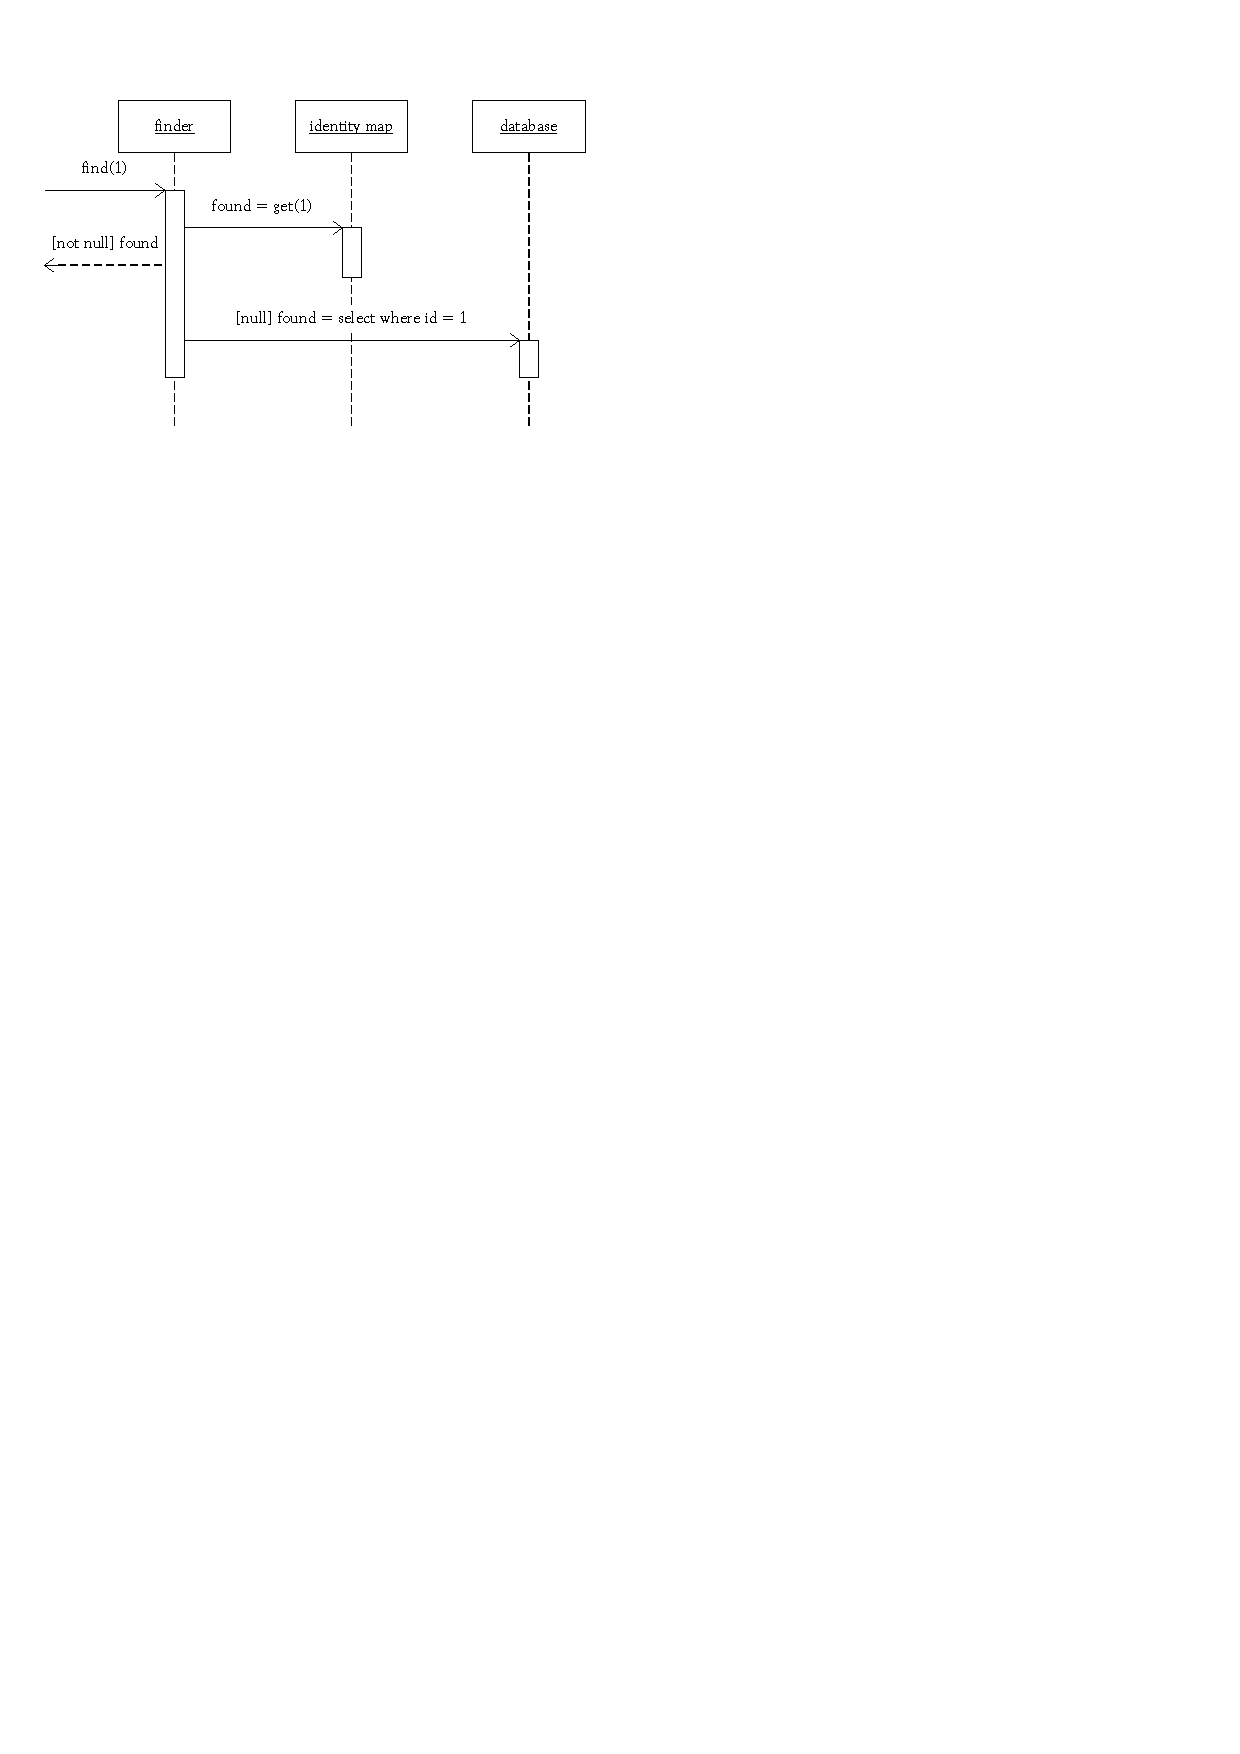
\includegraphics{./files/inc/figures/patternsIdentityMap}
					\caption{\label{fig:patternsIdentityMap} Mapping a collection to a foreign key}
				\end{center}
			\end{figure}

		\subsection{Lazy Load}
		\label{subsec:lazyLoad}
			If you load an object from the database into memory it is often useful to
			load objects that are related to it. This makes working with objects easier,
			because you don't have to load every single object yourself. The drawback of
			this mechanism is that it can have the effect of loading a huge number of
			related objects. This in turn can hurt the performance of your application
			drastically, especially when only a few objects are actually needed.
			\textit{Lazy Load} interrupts this loading process and leaves a marker in the
			object structure so that it can be loaded only 
			when it is used. This is shown in Figure \ref{fig:patternsLazyLoad1}.

			\begin{figure}[htb]
				\begin{center}
					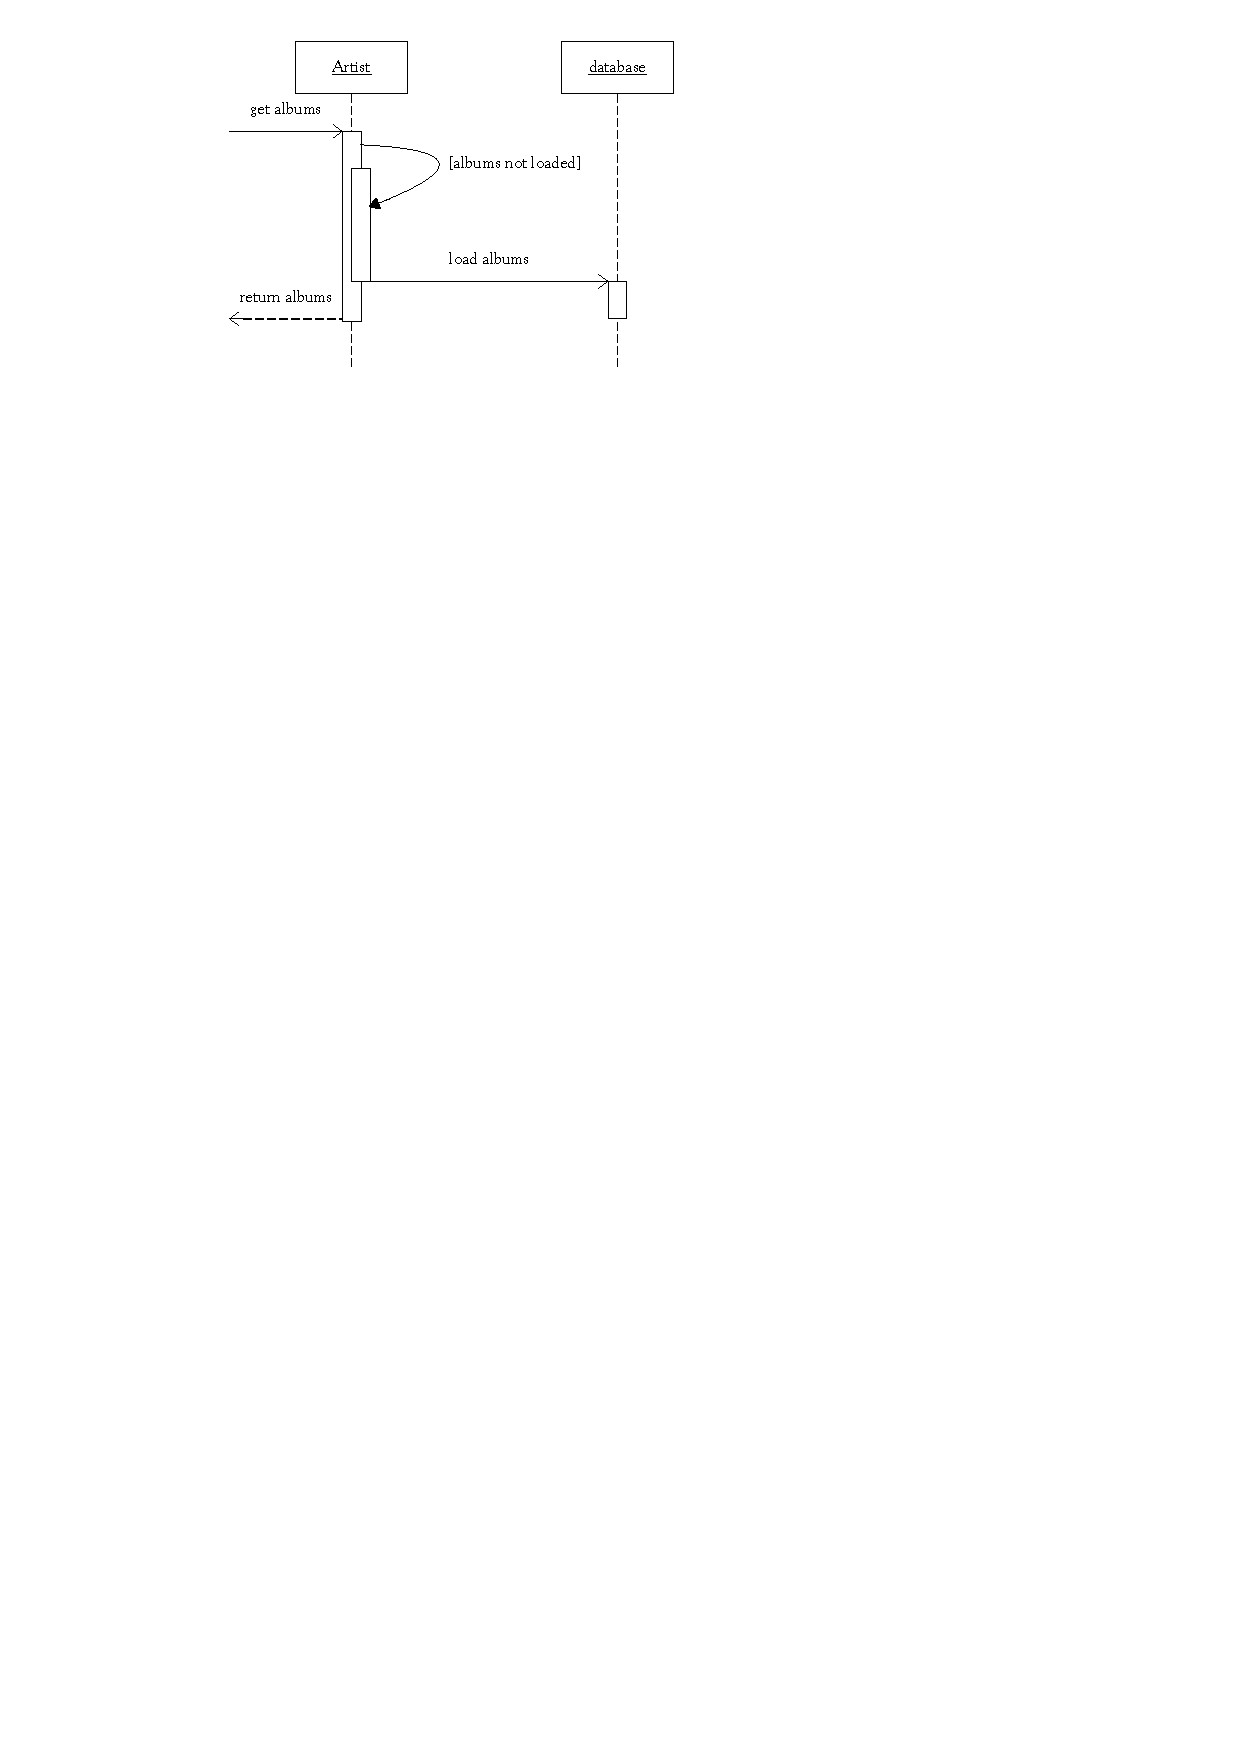
\includegraphics{./files/inc/figures/patternsLazyLoad1}
					\caption{\label{fig:patternsLazyLoad1} Sample Lazy Load Sequence}
				\end{center}
			\end{figure}
			Using \textit{Lazy Load} does not always improve performance. For instance, if
			you need to load all related objects, Lazy Load can even make performance
			worse that it was without it.

			There are four ways for implementing \textit{Lazy Load}
			\begin{itemize}
				\item Lazy Initialisation
				\item Virtual Proxy
				\item Value Holder
				\item Ghost
			\end{itemize}
			All of this methods have their own benefits and drawbacks but for the purpose of
			this thesis, a \textit{Virtual Proxy} pattern seems the most powerful and appropriate. A \textit{Virtual
			Proxy} is an object that looks like a real object but does not contain any data. Only when
			one of its methods is called does it load the correct object from the database. This pattern is
			described in E. Gamma's Design Patterns \cite{Gamma97}.
			
		\subsection{Unit of Work}
		\label{subsec:unitOfWork}
			It is important to know what you change in your domain model in order to apply those
			changes to the database. A \textit{Unit of Work} keeps track of what you have done
			during a business transaction and figures out what needs to be done to get the
			database in a consistent state. Therefore, a \textit{Unit of Word} needs to be informed
			every time an object is change, created or deleted. There are different ways to
			implement this. Either the user of an object register the object with the 
			\textit{Unit of Work} and mark objects as dirty after making any changes or
			the \textit{Unit of Work} handles this by its own. The latter case is preferable
			because it is less fault-prone. Figure \ref{fig:patternsUnitOfWork} shows the 
			working mechanism of this pattern.
		
			\begin{figure}[htb]
				\begin{center}
					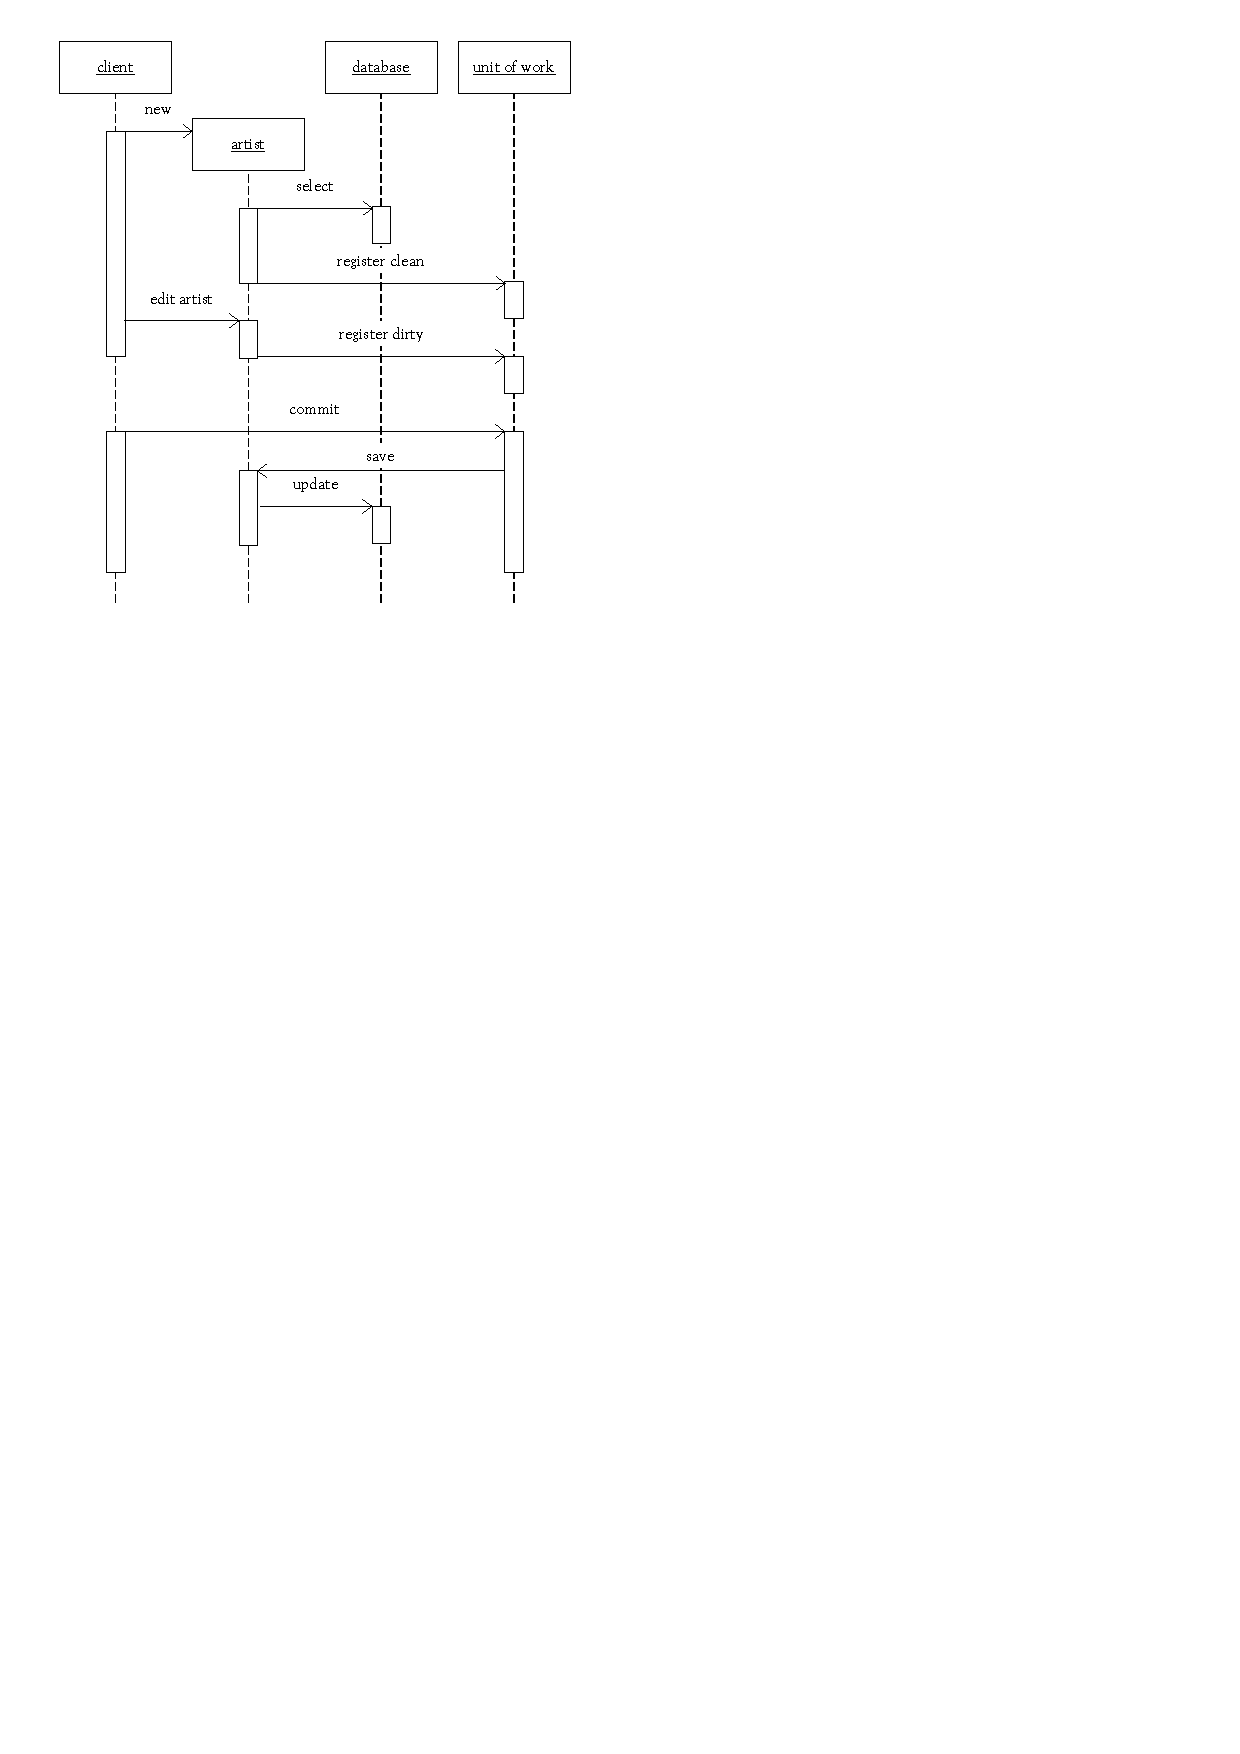
\includegraphics{./files/inc/figures/patternsUnitOfWork}
					\caption{\label{fig:patternsUnitOfWork} Unit of work mechanism}
				\end{center}
			\end{figure}
			
		\subsection{Foreign Key Mapping}
		\label{subsec:foreignKeyMapping}
			In an object-oriented system, objects are connected to each other directly or by object
			references. Relational databases use foreign key references for this. To save an object
			to a database, it is important to save these object references and map them to foreign 
			key references on the database. This is, what a \textit{Foreign Key Mapping} pattern does, it maps
			an object reference to a foreign key.

			These mappings can be of different kind and complexity. The simplest case is, if two
			objects are linked together. This association can be replaced
			by a foreign key in the database. This is shown in Figure \ref{fig:patternsForeignKeyMapping1}.

			\begin{figure}[htb]
				\begin{center}
					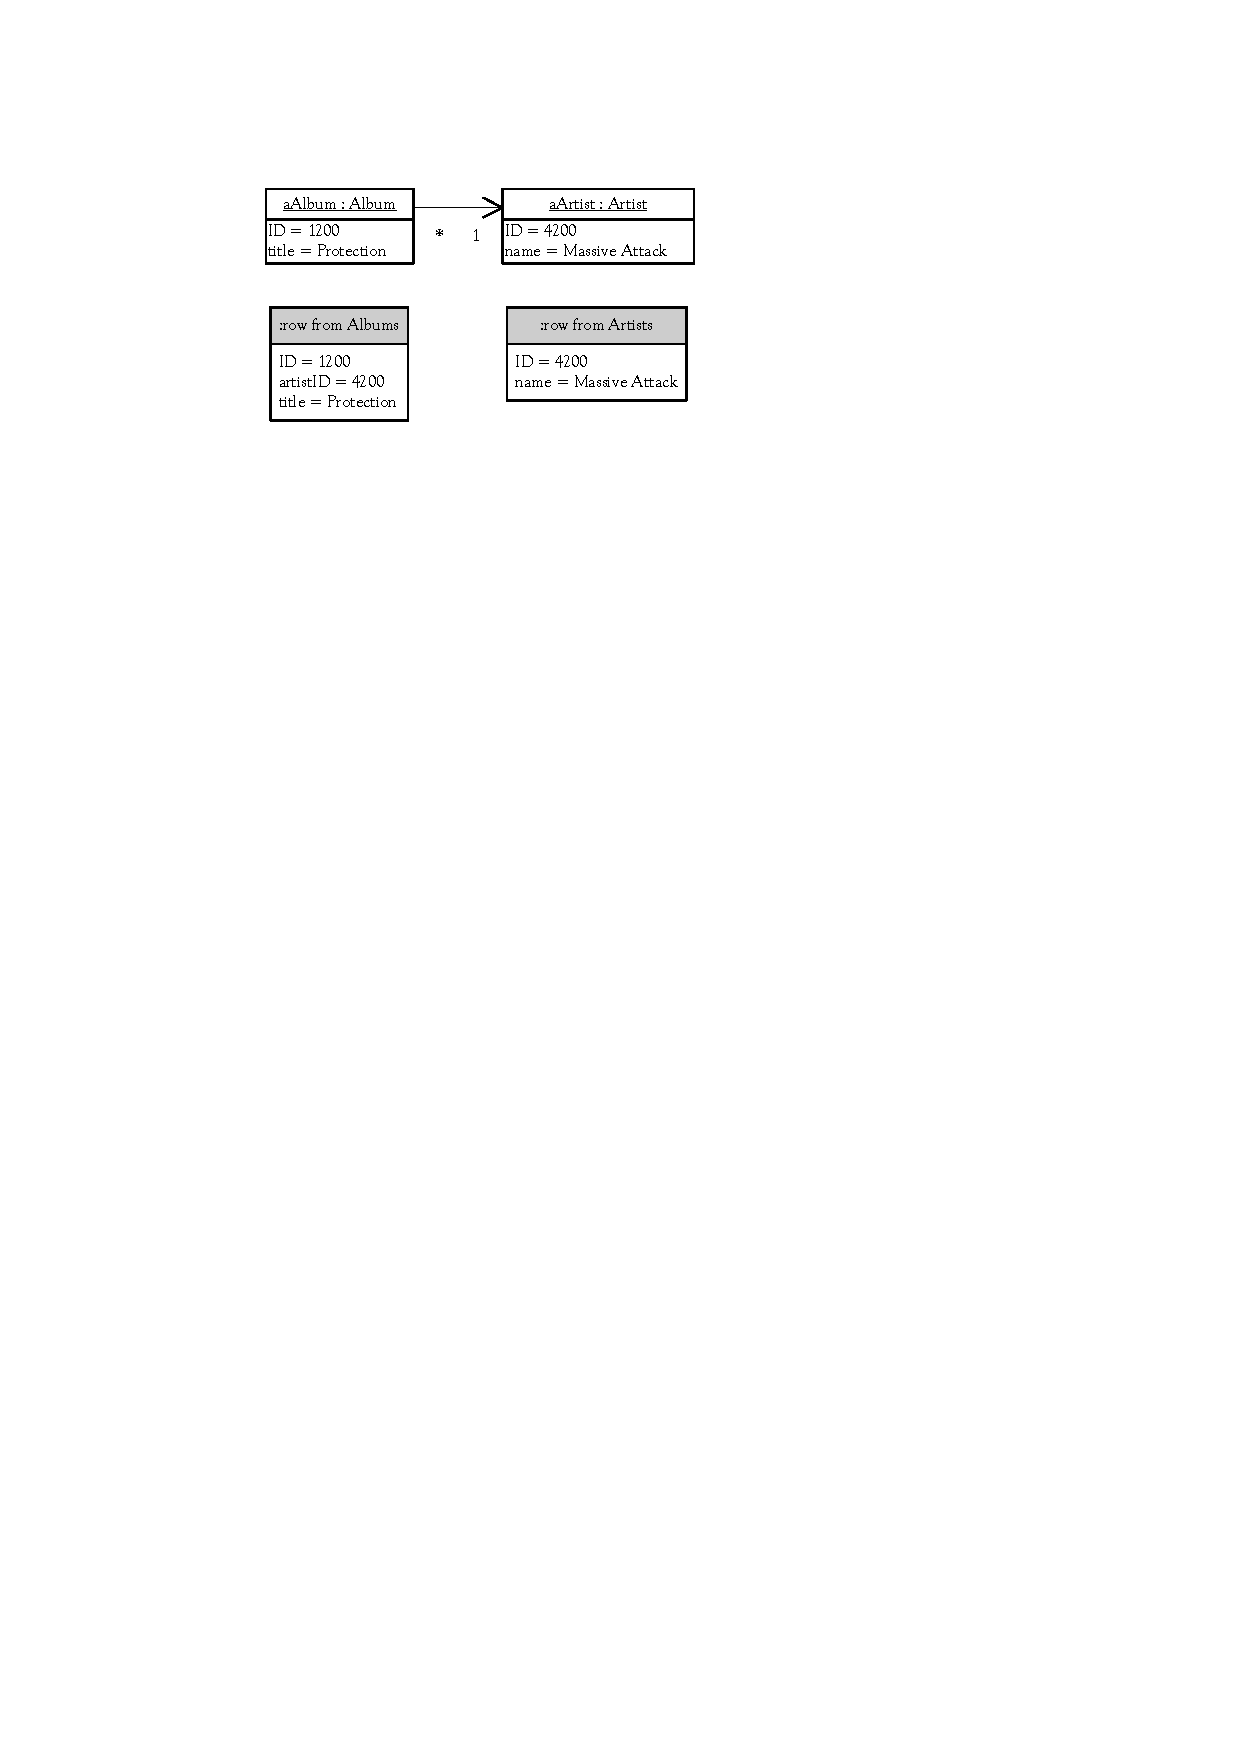
\includegraphics{./files/inc/figures/patternsForeignKeyMapping1}
					\caption{\label{fig:patternsForeignKeyMapping1} Simple Foreign Key Mapper}
				\end{center}
			\end{figure}
			Things get more complicated when one has to keep track of a collection of objects, because
			a collection cannot be saved to a database. The direction of the reference needs to be reversed.
			In our example, which is shown in Figure \ref{fig:patternsForeignKeyMapping2}, this means to
			store a foreign key of the album in the track record.

			\begin{figure}[htb]
				\begin{center}
					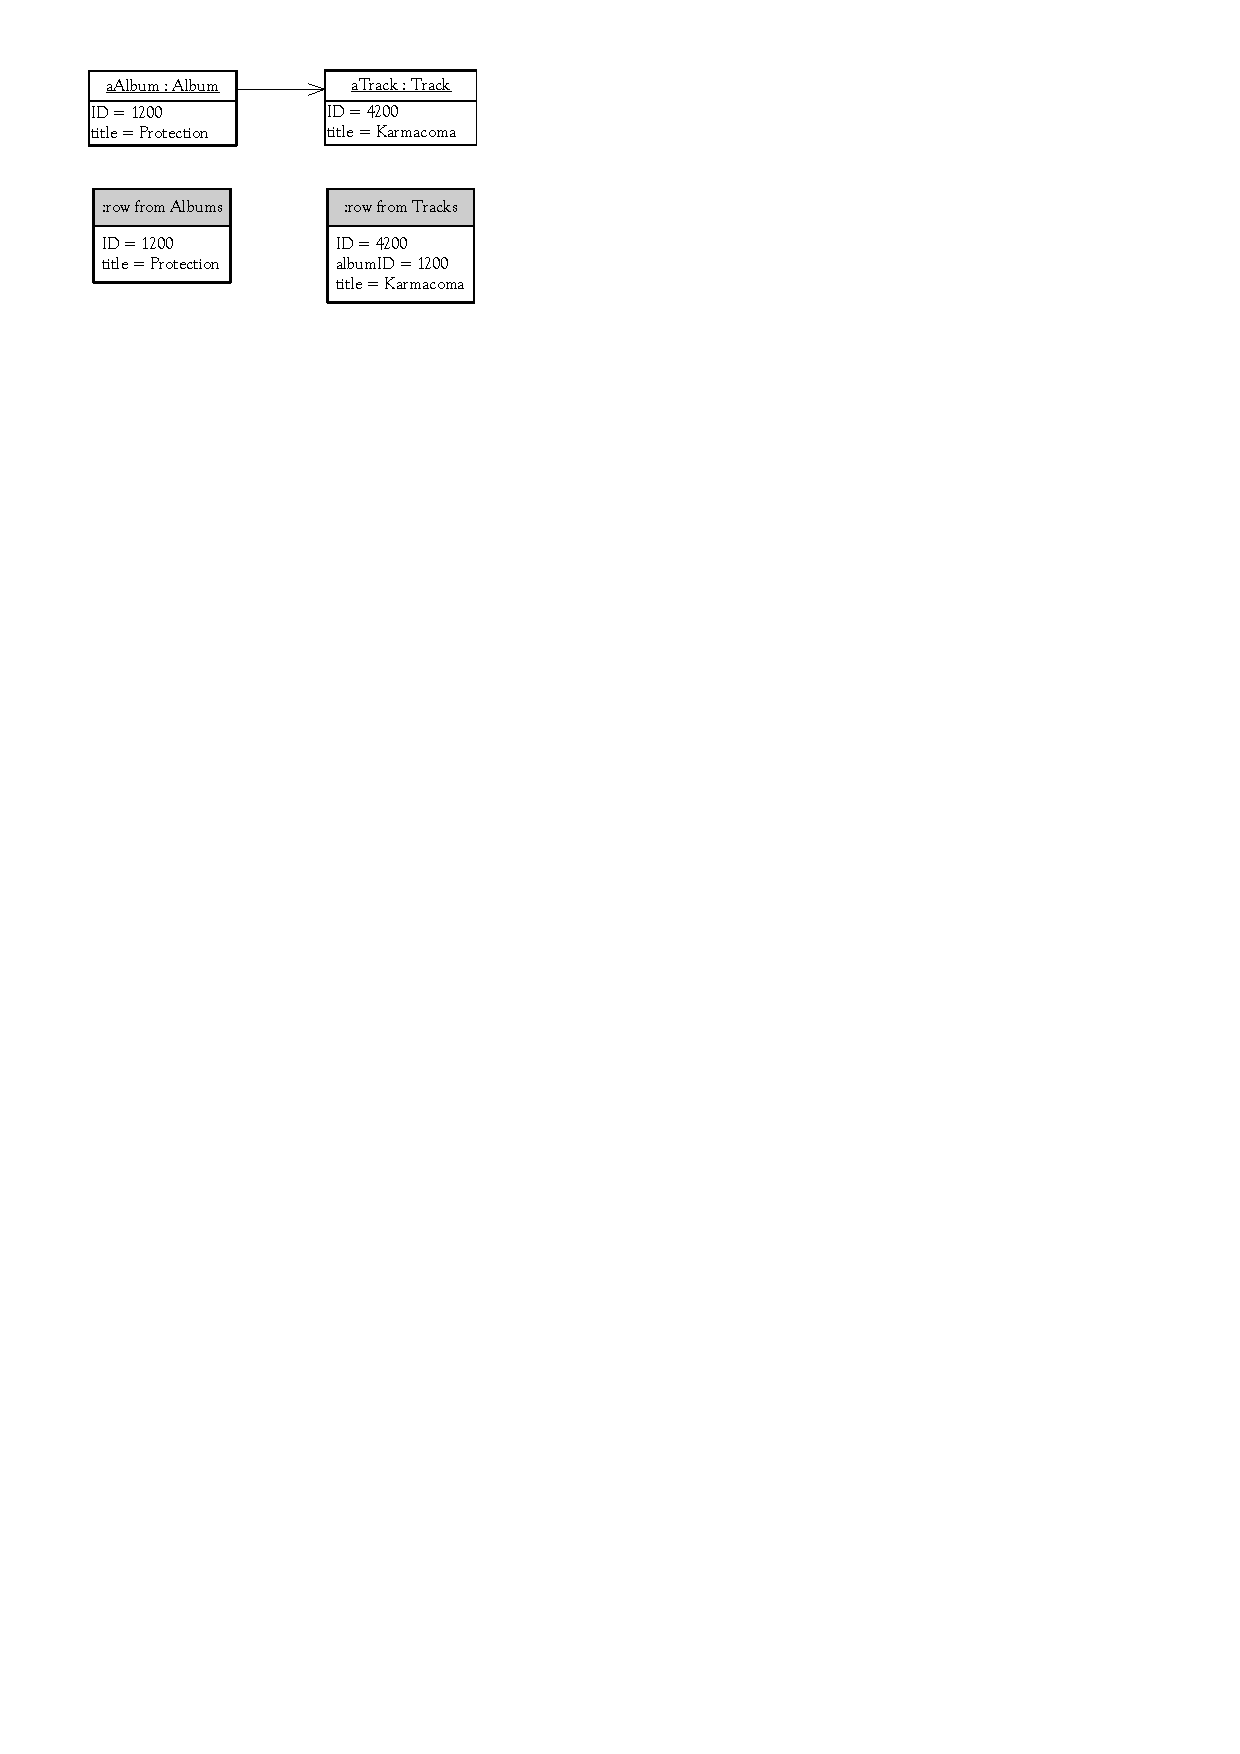
\includegraphics{./files/inc/figures/patternsForeignKeyMapping2}
					\caption{\label{fig:patternsForeignKeyMapping2} Mapping a collection to a foreign key}
				\end{center}
			\end{figure}
			This pattern needs to be discussed in more detail, especially cases where one needs
			to update a collection objects. This will be explained in the appropriate section, where
			implementation details are subjected.
			
		\subsection{Identity Field}
		\label{subsec:identityField}
			A relational database distinguishes one row from another by using keys. A key usually
			is nothing else than a \verb~long~ data-type. However, in-memory objects do not have such 
			key (it is the systems responsibility to keep track of object identities). Reading from a
			database is never a problem where database keys are concerned, writing is a problem though.
			One needs to save a copy of the database key in the in-memory object to tie this object to
			the corresponding database row. The \textit{Identity Field} pattern should be used whenever a mapping between
			in-memory objects and rows in a database is needed (which is almost always).
			
		\subsection{Metadata Mapping}
		\label{subsec:metadataMapping}
			As already mentioned, in-memory objects and database rows have different mechanisms to
			organise and structure data. Mapping this structures is what object-relational Mapping 
			is all about. To achieve this, many lines of code are needed to describe how fields in
			the database correspond to fields in in-memory objects. The resulting code
			is repetitive to write. With a code generation tool (in this case OOXGen - which is a result of this 
			thesis) a \textit{Metadata Mapping} pattern can be used to generate those repetitive lines of code.
			The input of the OOXGen is the metadata and the output is the source code of classes that do 
			the mapping. On most occasions the metadata is kept in a separate file, such as an XML file or
			even in the database itself. Figure \ref{fig:patternsMetadataMapping} shows the principle of the
			\textit{Metadata Mapping} pattern.
			
			\begin{figure}[htb]
				\begin{center}
					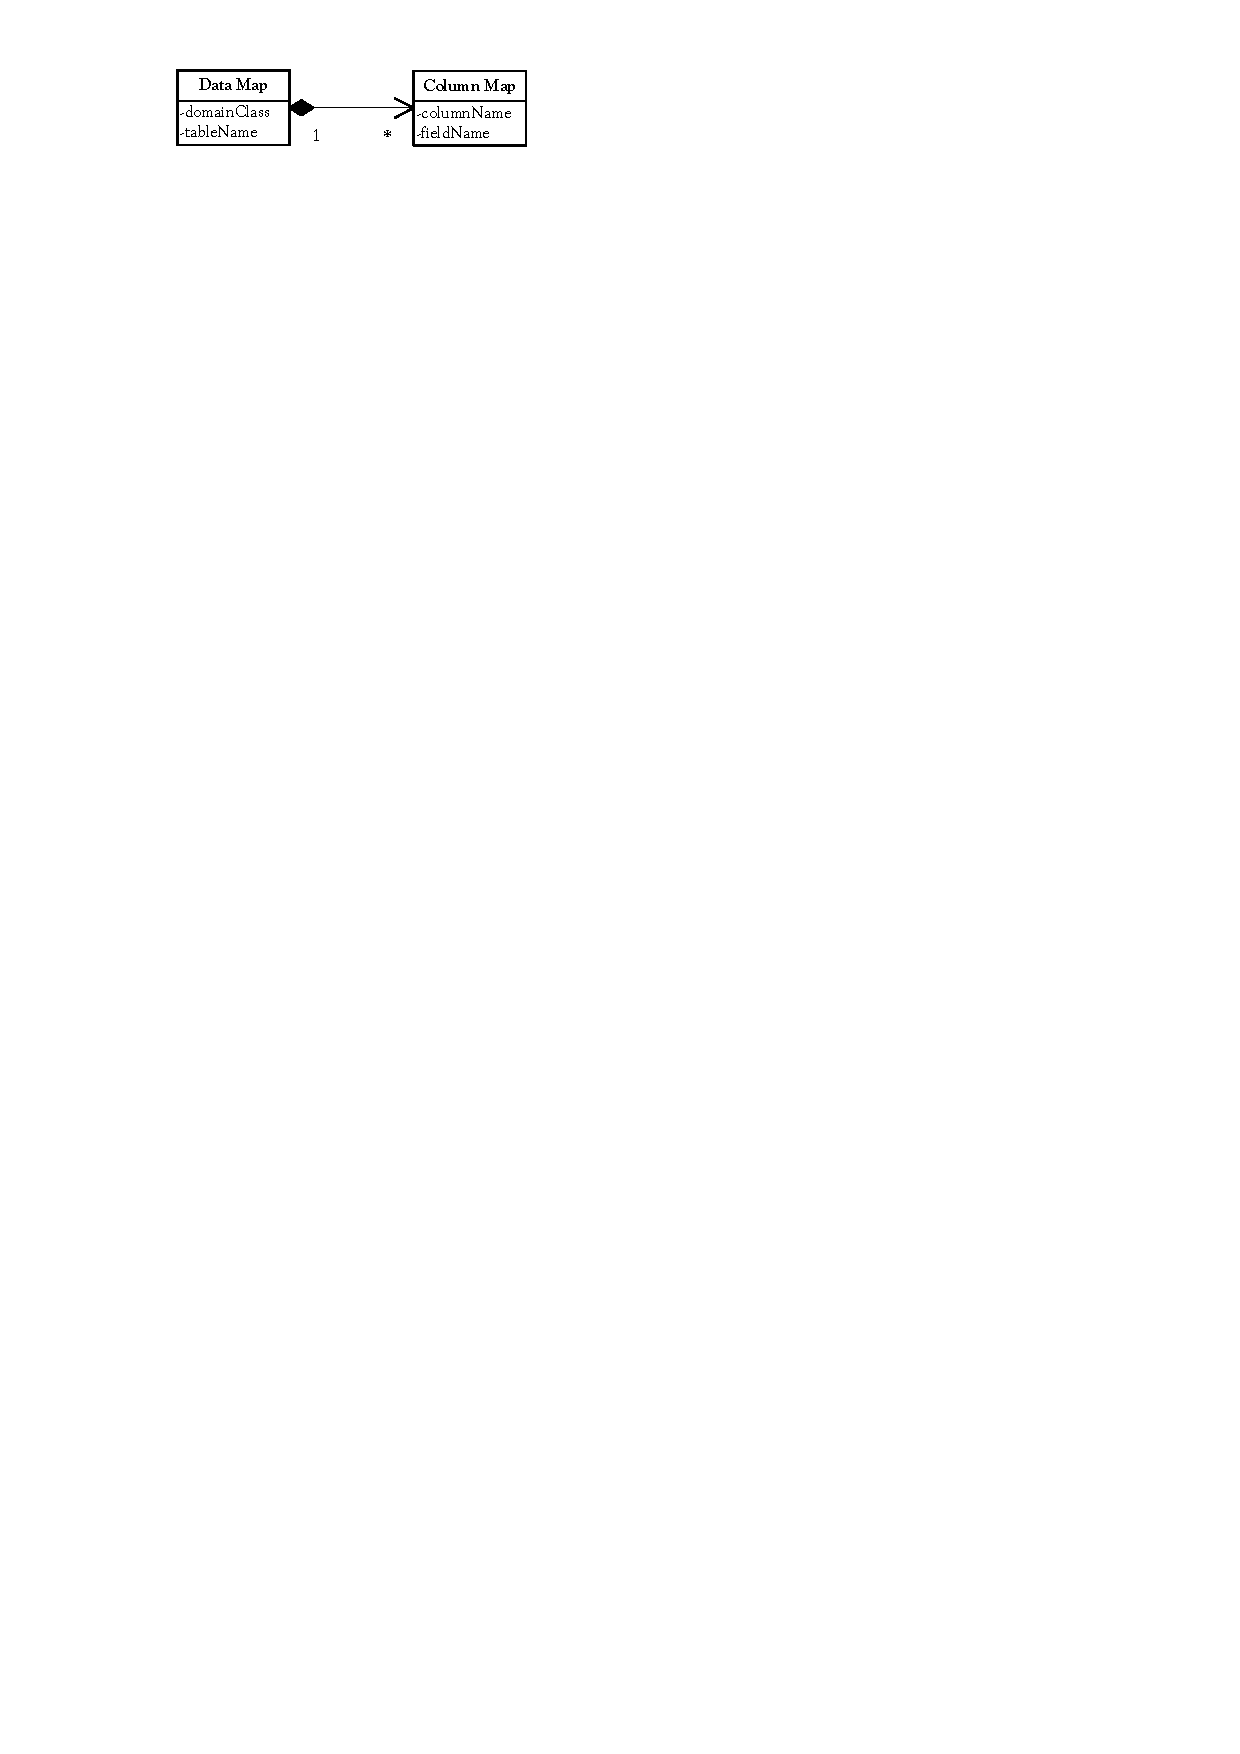
\includegraphics{./files/inc/figures/patternsMetadataMapping}
					\caption[Metadata Mapping principle]{\label{fig:patternsMetadataMapping} Holds details of object-relational mapping in metadata}
				\end{center}
			\end{figure}
			
		\subsection{Query Object}
		\label{subsec:queryObject}
			A \textit{Query Object} is a structure of objects that can form itself into a SQL query.
			A query can be formed by referencing classes and fields rather than tables and columns. 
			This allows a client to form a query of various kinds and turn those object structures into
			the appropriate SQL statement.
			With \textit{Query Object} you can separate SQL statements from the rest of the code
			which makes it possible to use different objects for different database schemata. This
			can be very powerful and makes code more readable. Furthermore a developer needs
			to know neither the details of the database nor he needs to be familiar with the SQL language.
			Figure \ref{fig:patternsQueryObject} shows an example of a possible \textit{Query Object}.
			
			\begin{figure}[htb]
				\begin{center}
					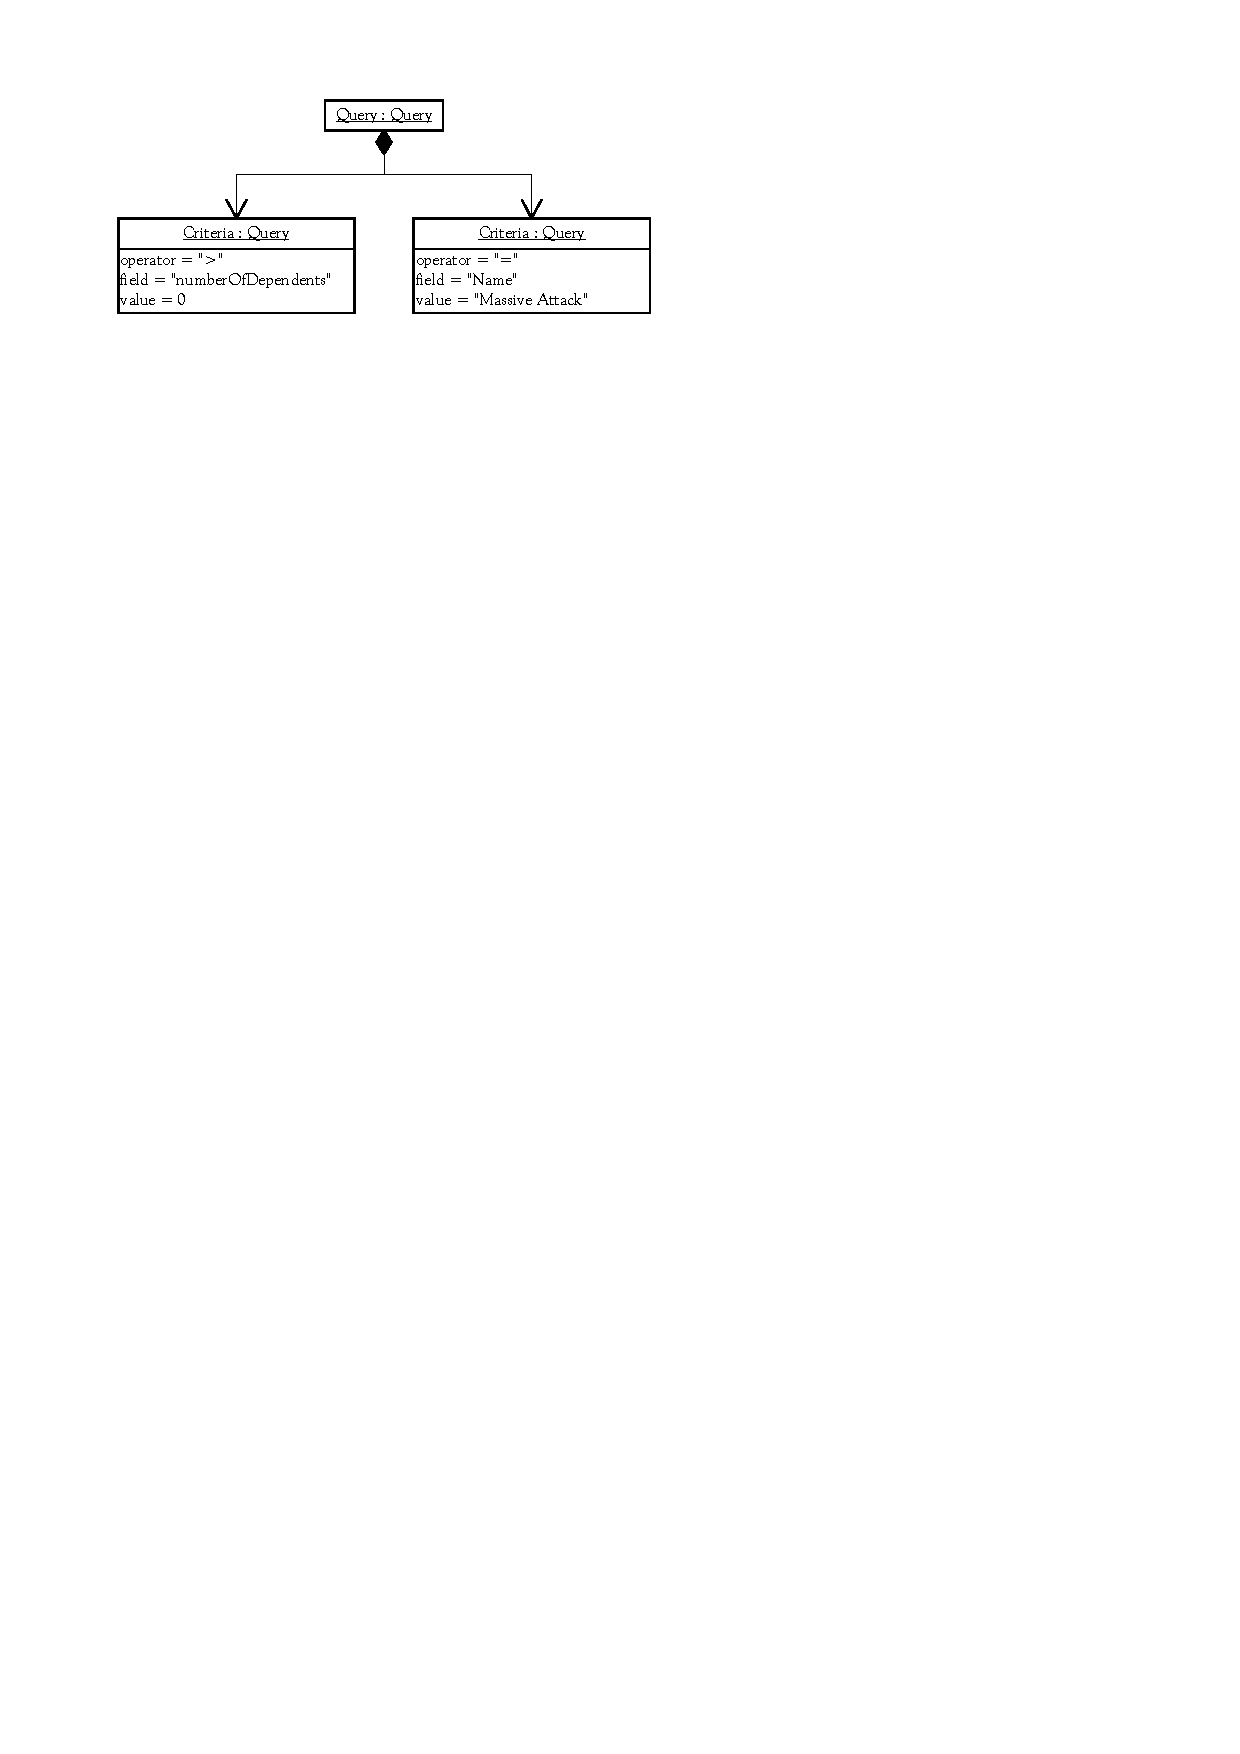
\includegraphics{./files/inc/figures/patternsQueryObject}
					\caption{\label{fig:patternsQueryObject} An Object Query representing a database query}
				\end{center}
			\end{figure}
			
		\subsection{Repository}
		\label{subsec:repository}
			A \textit{Repository} is a separation Layer between domain objects and a \textit{Data Mapper}.
			It isolates domain objects from details of the database access code. 
			Conceptually, a \textit{Repository}
			encapsulates the set of objects persisted in a data store and the operations performed over them.
			It presents a simple interface for clients which can create a Criteria object specifying
			the characteristics of the objects they want returned from a query. These Criteria Objects
			are submitted to the \textit{Repository} for satisfactory. In conjunction with 
			\textit{Query Object}, this pattern adds a large measure of 
			usability to the object-relational mapping layer. Client code do not need to use a \textit{Query Object}
			directly, instead it creates criteria objects and passes them to the \textit{Repository}, asking it 
			to select those objects that match.
			
		\subsection{Remote Facade}
		\label{subsec:remoteFacade}
			A remote call is always very expensive in terms of performance. It is better to do things in a
			single call rather than multiple calls. This is opposed to local calls. A \textit{Remote Facade}
			provides a coarse-grained interface for remote calls. This principle is illustrated in Figure
			\ref{fig:patternsRemoteFacade}. Rather than making a remote call for each element in an address,
			one call for all elements is performed. Therefore, this pattern describes the principle
			of designing coarse-grained interfaces which remote clients, such as web-services, can use.
			This pattern is a special \textit{Facade} which is described in E. Gamma's Design Patterns \cite{Gamma97}.
			A \textit{Facade} generally provides a simplified, standardised interface to a large set of objects.
			
			\begin{figure}[htb]
				\begin{center}
					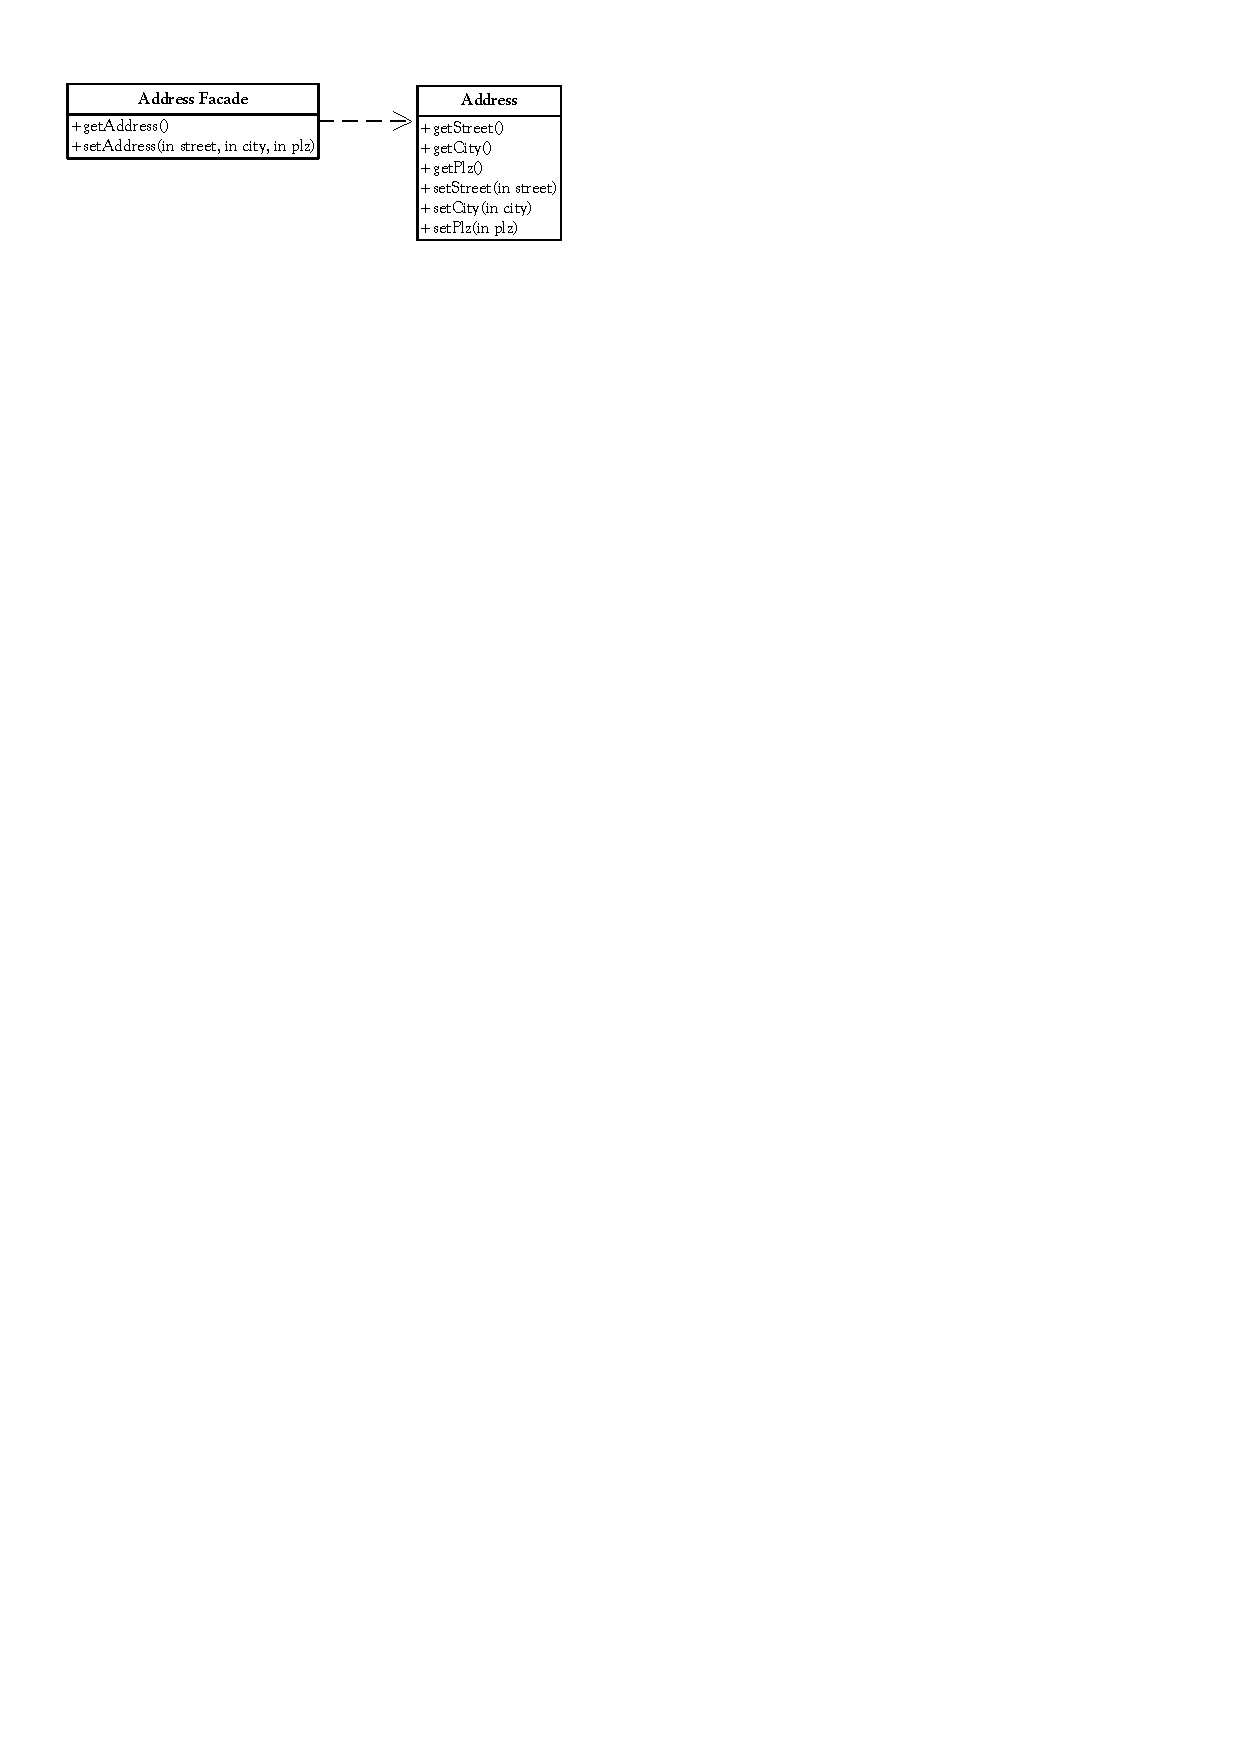
\includegraphics{./files/inc/figures/patternsRemoteFacade}
					\caption{\label{fig:patternsRemoteFacade} A coarse-grained remote call}
				\end{center}
			\end{figure}
			
		\subsection{Optimistic Offline Lock}
		\label{subsec:optimisticOfflineLock}
			A business transaction often includes a series of transaction. A single transaction
			is locked by the database manager. That is, no other transaction can access the same
			data at the same time. When you have more than a single transaction, you need a mechanism 
			to ensure that data at the end of a business transaction is in consistent state. This
			can be done with locks.
			There are two different approaches how a transaction can obtain a lock. This is
			either pessimistic or optimistic offline lock. The main difference is that \textit{Pessimistic
			Offline Lock} assumes that the chance of session conflict is high whereas \textit{Optimistic Offline
			Lock} assumes that the chance of one transaction conflicts with another is low. \textit{Pessimistic
			Offline Lock} is easier to implement but it limits system concurrency. This is because at a given time
			only one user can work with the locked data. \textit{Optimistic Offline Lock} allows multiple users to
			work with the same data at the same time. This is often very desirable but means to solve some problems
			which can occur when multiple users change data at the same time. Namely this problems are with
			\verb~UPDATE~ and \verb~DELETE~ SQL statements. Additionally, inconsistent reads must be detected.
			
			An \textit{Optimistic Offline Lock} is obtained by validating that, in the time since a transaction session loaded a
			record, another session has not altered it. This is usually done by comparing a version number
			stored in a session with the version in the record data.
			Figure \ref{fig:patternsOfflineLock} shows an \verb~UPDATE~ with \textit{Optimistic Offline Lock}. The version
			number is checked within the \verb~UPDATE~ statement and a row count of $1$ is returned in case of
			success otherwise a row count of $0$ is returned. An example of \textit{Optimistic Offline Lock} is 
			the concurrent versions system (CVS).
			
			\begin{figure}[htb]
				\begin{center}
					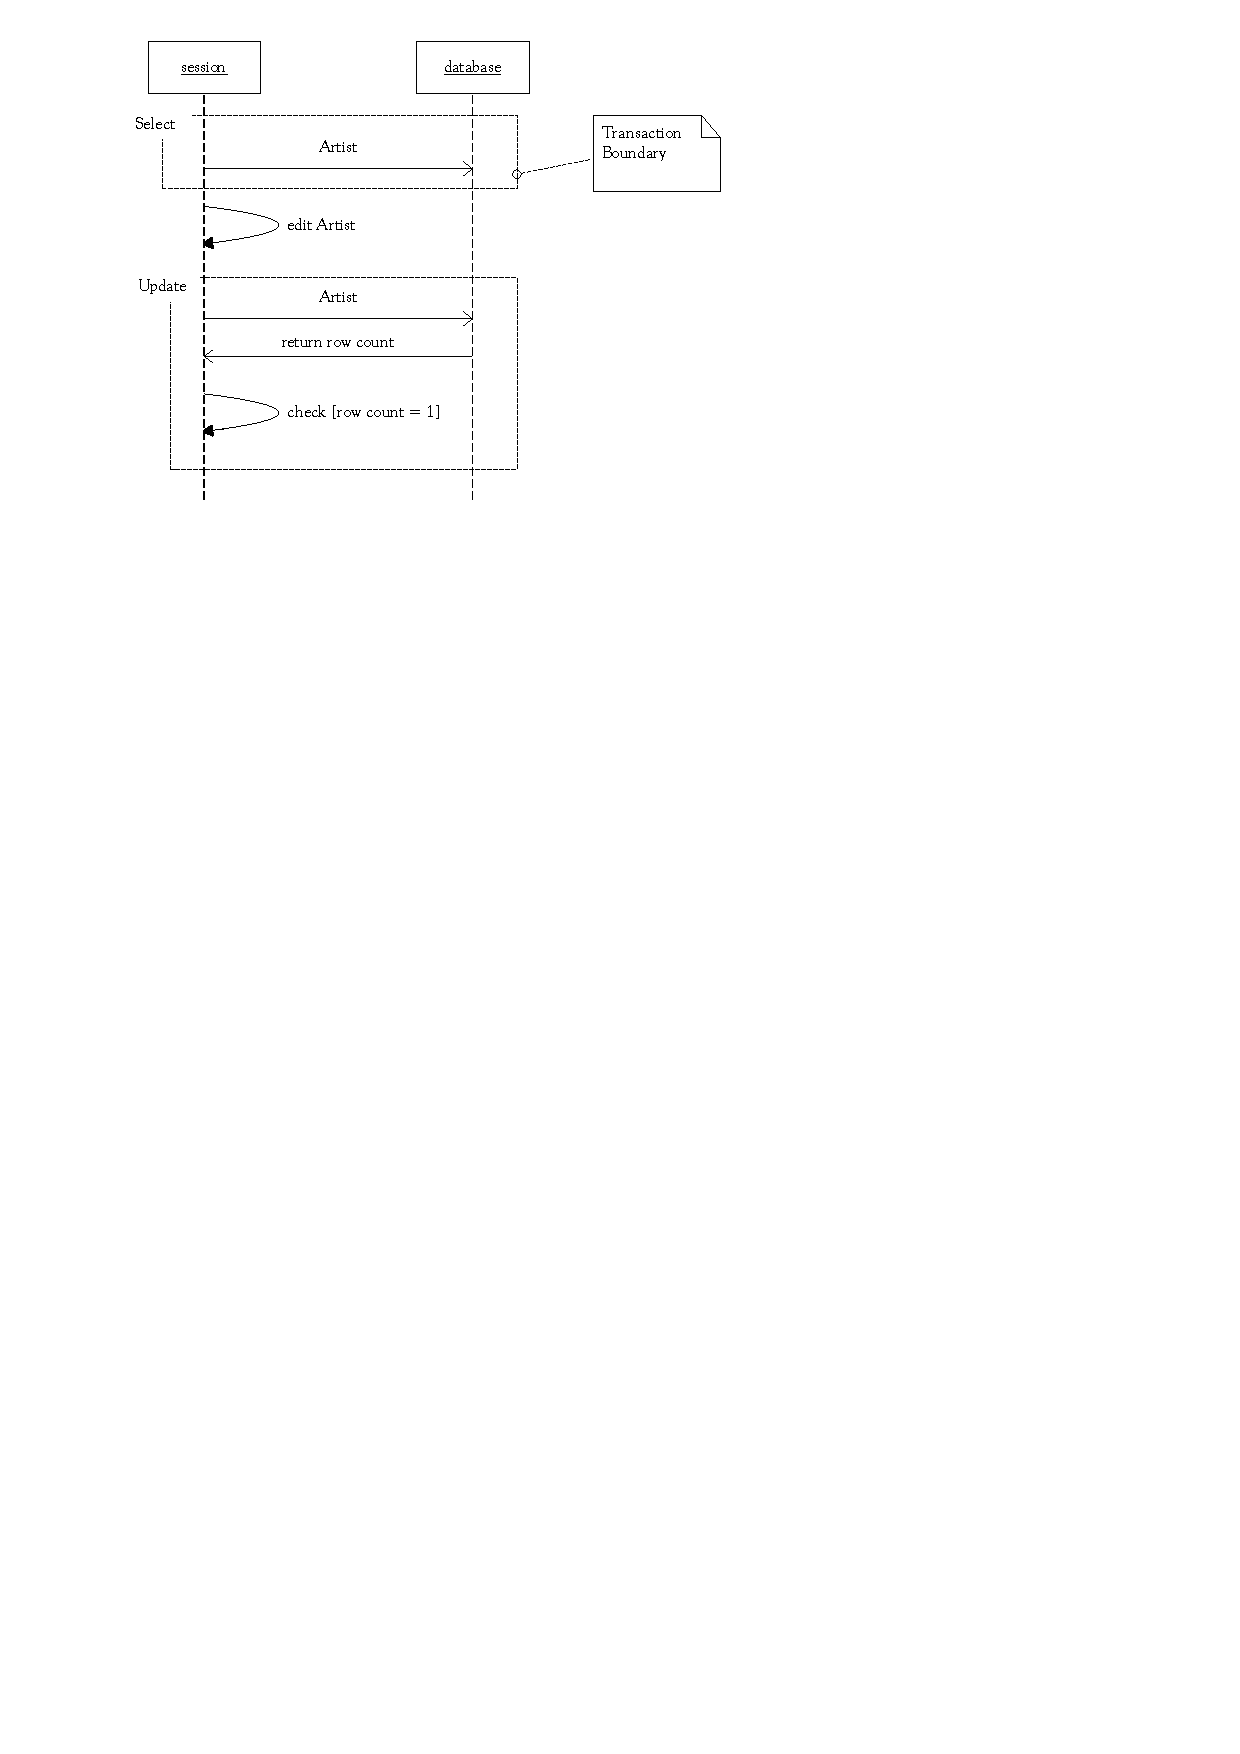
\includegraphics{./files/inc/figures/patternsOfflineLock}
					\caption{\label{fig:patternsOfflineLock} UPDATE with Optimistic Offline Lock}
				\end{center}
			\end{figure}
			Checks for inconsistent reads can become very tricky even with a few transactions. A 
			solution can be to group together transactions which depend on each other. This group 
			can be treated as a single lockable item.
			
		\subsection{Layer Supertype}
		\label{subsec:layerSupertype}
			The \textit{Layer Supertype} pattern describes the idea of an interface. An interface acts
			as a superclass which defines all common methods. Each class which references this 
			interface independently implements these methods.

			This way of implementing common features is very widespread in object-oriented
			programming and is therefore not explained in more detail.

		\subsection{Mapper}
		\label{subsec:mapper}
			A \textit{Mapper} is a layer between subsystems. It decouples these subsystems from each other. When
			using a \textit{Mapper}, either subsystem is not aware of the other but they still can communicate
			through the \textit{Mapper}. The most common case of a mapping layer is a \textit{Data Mapper}
			(\ref{subsec:dataMapper}).
				
		\subsection{Registry}
		\label{subsec:registry}
			A \textit{Registry} is essentially a global object. If you have methods for which
			you do not have a reference to start with, you can register this methods in a
			\textit{Registry}. A \textit{Registry} is usually implemented as a singleton class. This 
			makes it possible to get access to those methods from within the whole program. There are
			always workarounds in case you do not like to use a \textit{Registry}.
			
		\subsection{FactoryMethod}
		\label{subsec:factoryMethod}
			A \textit{Factory Method} defines an interface for creating an object. Which object
			is to be created is decided by subclasses. Usually a \textit{Factory Method} is needed
			when a class cannot anticipate the class of objects it must create. This is often the
			case with frameworks which must provide a mechanism to create concrete implementations
			of abstract classes. A framework does not know at design time which classes this will be.
			The idea is to pass all needed information to the \textit{Factory Method} which in turn
			will create the object. The advantage is to eliminate the need to bind application-specific
			classes into the code.
			The design of a \textit{Factory Method} is shown in Figure \ref{fig:patternsFactoryMethod}.
			
			\begin{figure}[htb]
				\begin{center}
					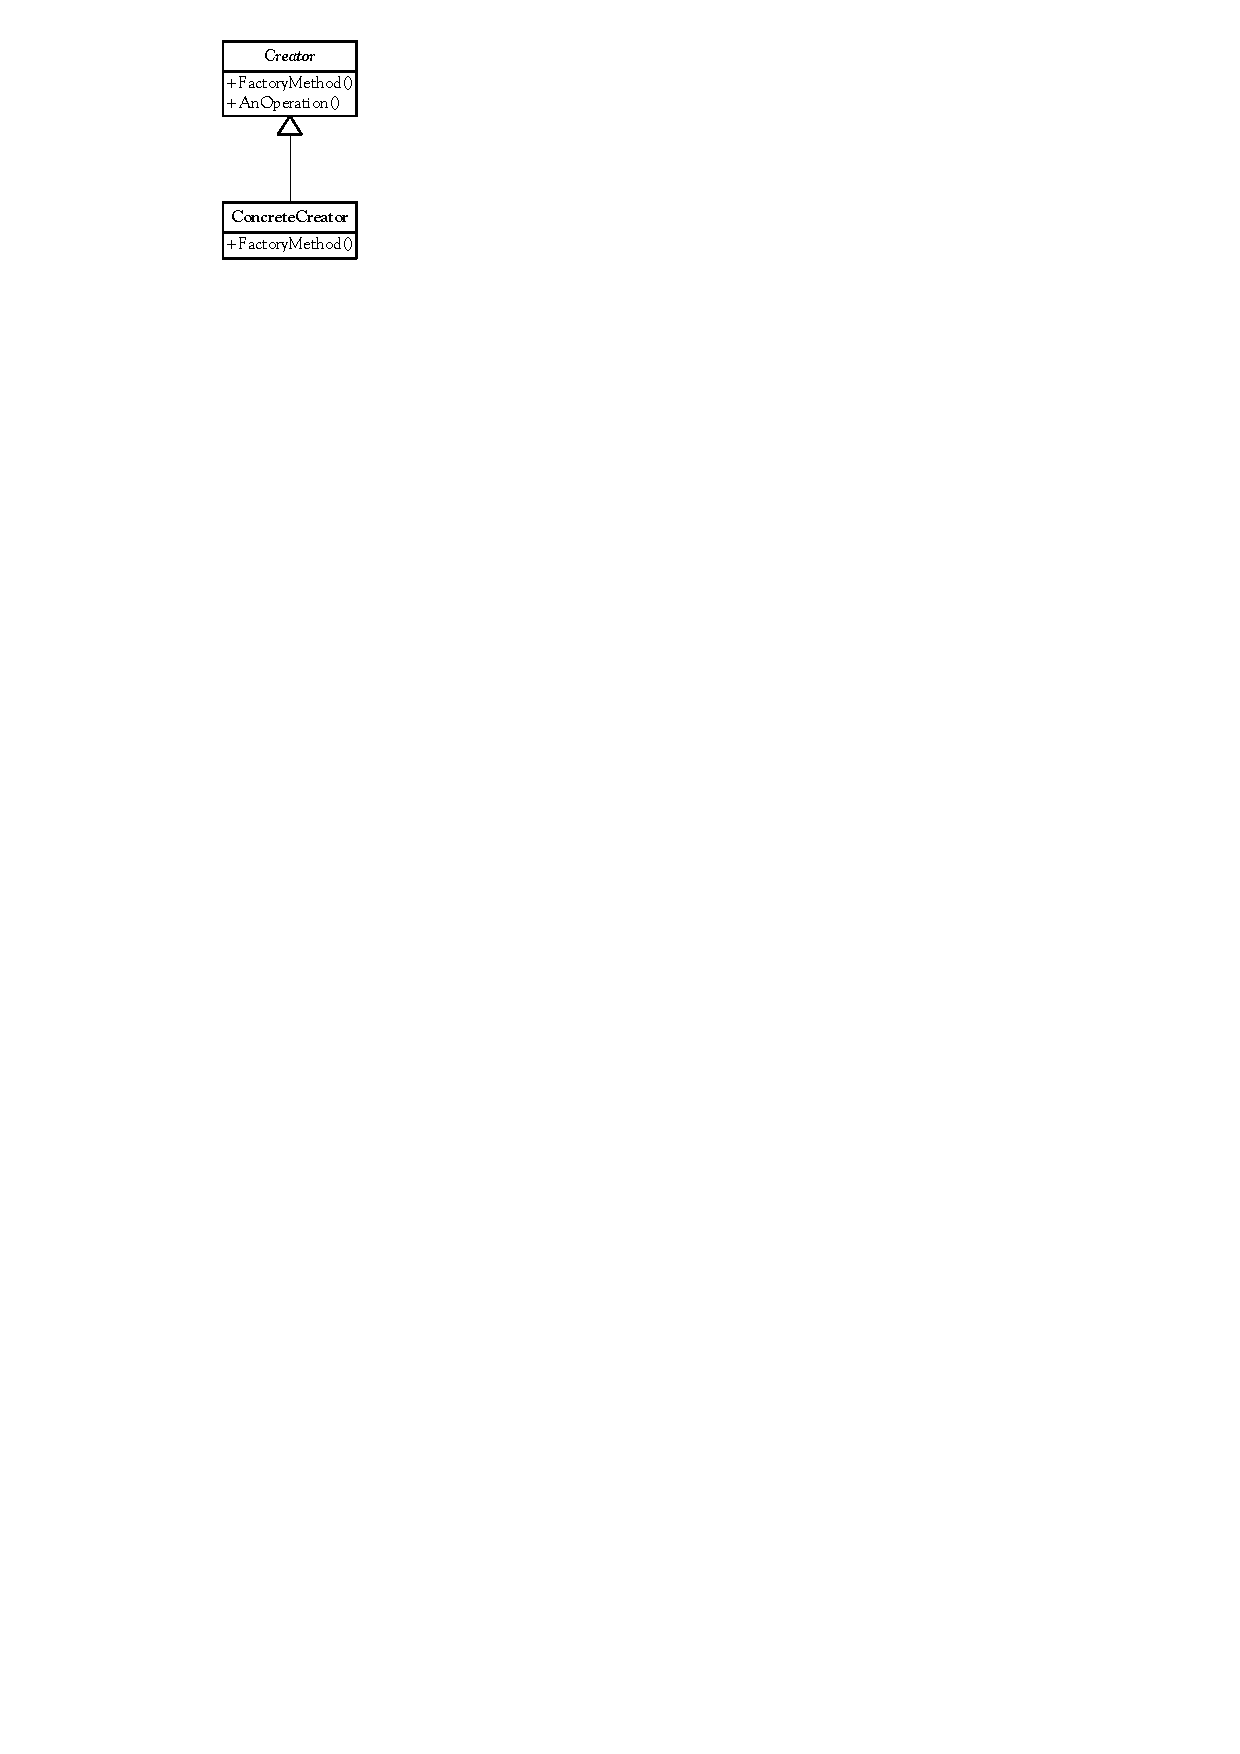
\includegraphics{./files/inc/figures/patternsFactoryMethod}
					\caption{\label{fig:patternsFactoryMethod} Factory Method Design}
				\end{center}
			\end{figure}

			
		\subsection{Separated Interface}
		\label{subsec:separatedInterface}
			A design paradigm is to decoupling individual parts of the system. A way to achieve this is
			to group classes in packages and control the dependencies between them. \textit{Separated Interface}
			is a way to manage these dependencies. You can define an interface in one package and put
			the implementation of this interface in a different package. This way, you do not have to
			reference classes in a different package, you only need a reference to the interface.
			A sample of this pattern is shown in Figure \ref{fig:patternsSeparatedInterface}
		
			\begin{figure}[htb]
				\begin{center}
					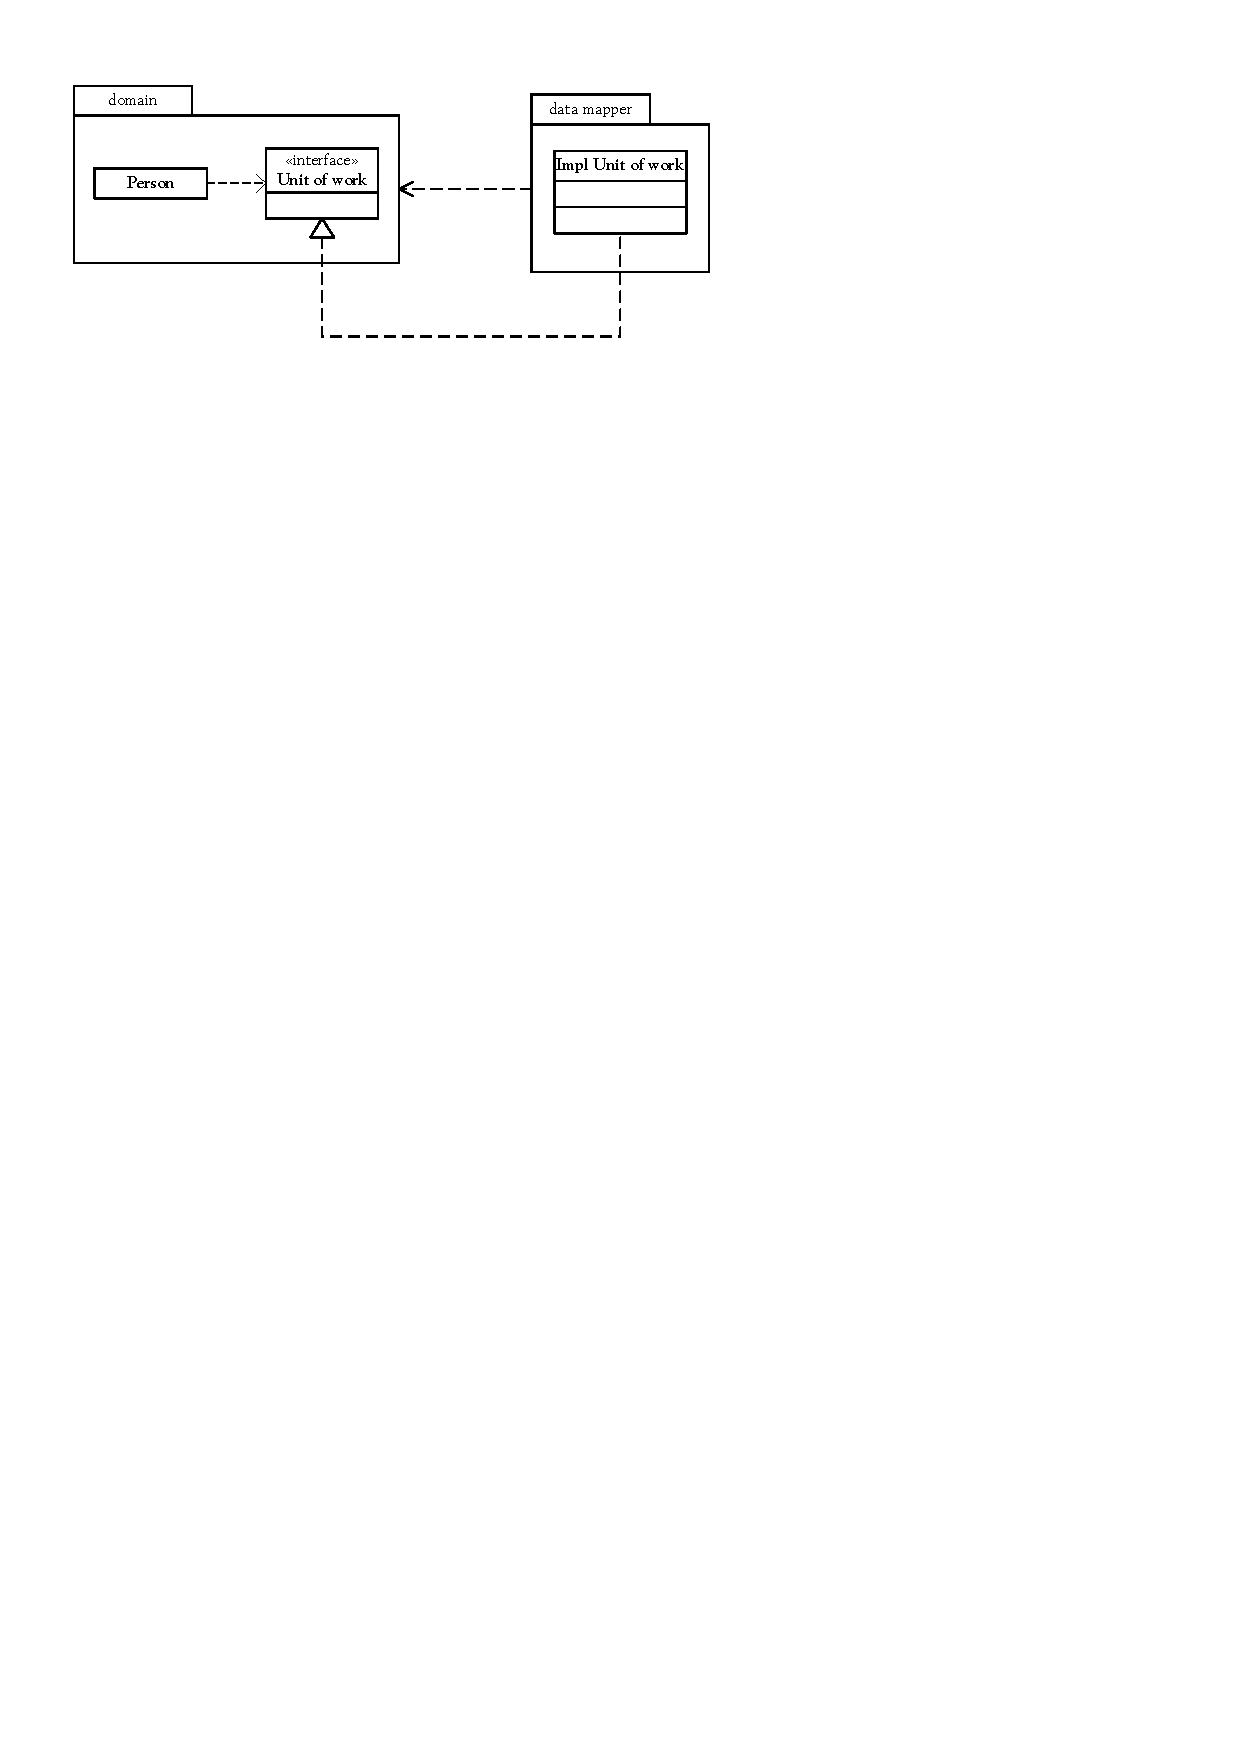
\includegraphics{./files/inc/figures/patternsSeparatedInterface}
					\caption{\label{fig:patternsSeparatedInterface} Sample of Separated Interface}
				\end{center}
			\end{figure}
